\chapter{CFG} \label{chap:appa}
\begin{lstlisting}[language=scriptkid, label={list:BNFCFG},caption=Context-free grammar for \lang in BNF form]
Program -> Cmds   
Cmds -> Cmd Cmds | EPSILON   
Cmd -> Stmt | Dcl   
Dcl -> Type Id Ass ;   
Ass -> = Expr | EPSILON   
Stmt -> Id = Expr ; | CtrlStrct | ListStmt ; | FuncDef | FuncCall ; | CommentStmt ; | return Type ; 
Expr -> LogicOr OprOr   
OprOr -> or LogicOr OprOr | EPSILON   
LogicOr -> LogicAnd OprAnd   
OprAnd -> and LogicAnd OprAnd | EPSILON   
LogicAnd -> Equal OprEql   
OprEql -> is Equal OprEql | is not Equal OprEql | EPSILON   
Equal -> Bool OprBool   
OprBool -> > Bool OprBool | < Bool OprBool | >= Bool OprBool | <= Bool OprBool | EPSILON   
Bool -> Term OprExpr   
OprExpr -> + Term OprExpr | - Term OprExpr | EPSILON   
Term -> Factor OprTerm   
OprTerm -> * Factor OprTerm | / Factor OprTerm | EPSILON 
Factor -> ( Expr ) | FuncCall | ListOprExpr | Num | Decimal | String | Id | Boolean 
Block -> { Cmds } 
CommentStmt -> comment: StringChars 
CtrlStrct -> IfStmt | Loop   
IfStmt -> if ( Expr ) Block ElseIfStmt   
ElseIfStmt -> else if ( Expr ) Block ElseIfStmt | Else | EPSILON   
Else -> else Block   
Loop -> repeat Loops   
Loops -> LoopStmt | WhileStmt | ForeachStmt   
LoopStmt -> ( Expr ) times Block 
WhileStmt -> while ( Expr ) Block   
ForeachStmt -> for each ( Type Id in Id ) Block   
ListStmt -> ListOpr | ListOprExpr 
ListOpr -> Id : Add ( ArgList ) | Id : Replace ( ArgList ) 
ListOprExpr -> Id : IndexOf ( Expr ) | Id : ValueOf ( ArgList ) 
FuncCall -> call Id ( ArgList ) | call output ( ArgList ) | call Type input ( ArgList ) 
FuncDef -> function Id ( ParamList ) FuncReturn Block   
FuncReturn -> return FuncReturnType   
FuncReturnType -> Type | nothing   
ParamList -> Param ParamTail | EPSILON   
ParamTail -> , Param ParamTail | EPSILON   
Param -> Type Id   
ArgList -> Expr ArgTail | EPSILON   
ArgTail -> , Expr ArgTail | EPSILON   
Boolean -> true | false   
Type -> boolean | text | number | decimal | list ( Type )   
Id -> Letter Chars 
String -> '"' StringChars '"'  
StringChars -> StringChar StringChars | EPSILON 
StringChar -> Char | SpecialChar  
Chars -> Char Chars | EPSILON  
Char -> Digit | Letter   
Letters -> Letter Letters | EPSILON   
Letter -> a ... z | A ... Z | _   
Decimal -> Num . Num 
Num -> Digit Digits   
Digits -> Digit Digits | EPSILON   
Digit -> 0 ... 9 
SpecialChar -> ! | @ | # | £ | ¤ | $ | % | & | / | ( | ) | { | } | [ | ] | = | ? | + | - | ` | ^ | ~ | * | , | . | ~ | § | ½ 
\end{lstlisting}  


\chapter{ANTLR CFG + LEXER}
\begin{lstlisting}[language=scriptkid, label={list:ANTLRCFG},caption=Context-free grammar for \lang used in ANTLR]
    program: cmds;  
cmds: cmd cmds | /*epsilon*/;  
cmd: stmt | dcl;  
dcl: type ID ass SEMI;  
ass: ASSIGN expr | /*epsilon*/;   
stmt: ID ASSIGN expr SEMI |  
ctrlStrct |  
listStmt SEMI | 
funcDef | 
funcCall SEMI | 
commentStmt SEMI | 
RETURN type SEMI;   
expr: logicOr oprOr;  
oprOr: OR logicOr oprOr | /*epsilon*/;  
logicOr: logicAnd oprAnd;  
oprAnd: AND logicAnd oprAnd | /*epsilon*/;  
logicAnd: equal oprEql;  
oprEql: EQUAL equal oprEql | NOT equal oprEql | /*epsilon*/;  
equal: bool oprBool;  
oprBool: GREAT bool oprBool | LESS bool oprBool |   
GREATEQL bool oprBool| LESSEQL bool oprBool | /*epsilon*/;  
bool: term oprExpr;  
oprExpr: ADD term oprExpr | SUB term oprExpr | /*epsilon*/;  
term: factor oprTerm; 
oprTerm: MUL factor oprTerm | DIV factor oprTerm | /*epsilon*/;  
factor: LPAREN expr RPAREN | funcCall | listOprExpr | INT | DEC | STR | ID | boolean;  
block: LCURLY cmds RCURLY;  
commentStmt: COMM; 
ctrlStrct: ifStmt | loop; 
ifStmt: IF LPAREN expr RPAREN block elseIfStmt;  
elseIfStmt: ELSE IF LPAREN expr RPAREN block elseIfStmt | else |  
/*epsilon*/;  
else: ELSE block;   
loop: REPEAT loops; 
loops: loopStmt | whileStmt | foreachStmt; 
loopStmt: LPAREN expr RPAREN TIMES block; 
whileStmt: WHILE LPAREN expr RPAREN block; 
foreachStmt: FOREACH LPAREN type ID IN ID RPAREN block; 
listStmt: listOpr | listOprExpr; 
listOpr: ID COLON LISTADD LPAREN argList RPAREN |  
ID COLON LISTDEL LPAREN argList RPAREN; 
listOprExpr: ID COLON LISTIDXOF LPAREN argList RPAREN |  
ID COLON LISTVALOF LPAREN argList RPAREN; 
funcCall: CALL ID LPAREN argList RPAREN |  
CALL PRINT LPAREN argList RPAREN |  
CALL type SCAN LPAREN argList RPAREN; 
funcDef: FUNCTION ID LPAREN paramList RPAREN funcReturn block; 
funcReturn: RETURN funcReturnType; 
funcReturnType: type | NOTHING; 
paramList: param paramTail | /*epsilon*/; 
paramTail: COMMA param paramTail | /*epsilon*/; 
param: type ID; 
argList: expr argTail | /*epsilon*/; 
argTail: COMMA expr argTail | /*epsilon*/; 
boolean: TRUE | FALSE;  
type: BOOL | TEXT | NUM | LIST LPAREN type RPAREN | DECIMAL; 
\end{lstlisting}



\begin{lstlisting}[label={list:ANTLR LEXER},caption=Lexer for \lang used in the ANTLR CFG]
OR: 'or'; 
AND: 'and'; 
EQUAL: 'is'; 
NOT: 'is not'; 
GREAT: '>'; 
LESS: '<'; 
GREATEQL: '>='; 
LESSEQL: '<='; 

ASSIGN : '=' ; 
COMMA : ',' ; 
SEMI : ';' ;
COLON: ':';
LPAREN : '(' ; 
RPAREN : ')' ; 
LCURLY : '{' ; 
RCURLY : '}' ; 
TRUE: 'true'; 
FALSE: 'false';

ADD: '+'; 
SUB: '-'; 
MUL: '*'; 
DIV: '/'; 
BOOL: 'boolean'; 
TEXT: 'text'; 
NUM: 'number';
DECIMAL: 'decimal';
NOTHING: 'nothing';
LIST: 'list';
QUOTE: '"'; 
IF: 'if'; 
ELSE: 'else';
REPEAT: 'repeat';
TIMES: 'times';
WHILE: 'while';
FOREACH: 'for each';
IN: 'in';
FUNCTION: 'function';
RETURN: 'return';
CALL: 'call';
PRINT: 'output';
SCAN: 'input';
COMMENT: 'comment:';

LISTADD: 'Add';
LISTIDXOF: 'IndexOf';
LISTREPLACE: 'Replace';
LISTVALOF: 'ValueOf';

COMM: 'comment:'~(';')*;
STR: '"' (~'"')* '"';
DEC: ('+' | '-')? [0-9]+'.'[0-9]+; 
INT: ('+' | '-')? [0-9]+ ;
ID: [a-zA-Z_][a-zA-Z_0-9]* ; 
WS: [ \t\n\r\f]+ -> skip ; 
\end{lstlisting}

\chapter{Type System} \label{Appendix:TypeSystem}

This appendix acts as a continuation of the Type system defined in section \ref{sec:TypeRules} \\

\section{Expression} \label{Appendix:Typesystem:Eq}

\begin{equation}
    (NUMEXP_{TS}) \ E\vdash n: number
\end{equation}

\begin{equation}
    (DECEXP_{TS}) \ E\vdash d: decimal
\end{equation}

\begin{equation}
    (TEXTEXP_{TS}) \ E\vdash txt: text
\end{equation}

\begin{equation}
    (BOOLEXP1_{TS}) \ E\vdash \mathbb{T} : boolean
\end{equation}

\begin{equation}
    (BOOLEXP2_{TS}) \ E\vdash \mathbb{F} : boolean
\end{equation}

\begin{equation}
   (VAREXP_{TS}) \frac{E\ (x)\ =\ T}{\ E\ \vdash \ x\ :\ T}
\end{equation}

\begin{equation}
    (PAREXP_{TS}) \frac{\ e\ :\ B}{\ E\ \vdash \ (e)\ :\ B}
\end{equation}

\begin{equation}
   (LISTSEXP_{TS}) \frac{E\ \vdash\ e\ :\ B }
    {\ E\ \vdash \  list (B)\ :\ ok} 
    \ for \ e \in L
\end{equation}

\begin{equation}
    (DEC*1_{TS})\frac{E \ \vdash \ e_1 : \ decimal \ E \ \vdash \ e_2 : \ number \ }{E \ \vdash e_1 \star \ e_2 \ : \ decimal} \ \ \ \
    where \ \star \in \{ +, *, - , /\}
\end{equation}

\begin{equation}
    (DEC*2_{TS})\frac{E \ \vdash \ e_1 : \ number \ E \ \vdash \ e_2 : \ decimal \ }{E \ \vdash e_1 \star \ e_2 \ : \ decimal} \ \ \ \
    where \ \star \in \{ +, *, - , /\}
\end{equation}

\begin{equation}
    (NUMDIV_{TS})\frac{E \ \vdash \ e_1 : \ number \ E \ \vdash \ e_2 : \ number \ }{E \ \vdash e_1 / \ e_2 \ : \ decimal}
\end{equation}



\begin{equation}
    (BOOL*_{TS})\frac{E \ \vdash \ e_1 : \ boolean \ E \ \vdash \ e_2 : \ boolean \ }
    {E \ \vdash e_1 \star \ e_2 \ : \ boolean} \ \ \ \
    where \ \star \in \{ and, \ or, \ is, \ is \ not\}
\end{equation}

\begin{equation}
    (TXT_{TS})\frac{E \ \vdash \ e_1 : \ text \ E \ \vdash \ e_2 : \ text \ }{E \ \vdash e_1 + \ e_2 \ : \ text} \  
\end{equation}

\section{Statements}
\begin{equation}
(LISTSTM1_{TS}) \frac{E\ \vdash x\ :\ list(B) \ \ E\ \vdash\ (x_1,...,x_k)\ :\ B }
{\ E\ \vdash \ x:Add(x_1, ...,\ x_k)\ :\ ok}
\end{equation}
\begin{equation}
    (LISTSTM2_{TS}) \frac{E\ \vdash\ x\ :\ list(B) \ \ \ E\ \vdash\ x_1\ :\ B \ \ \ E\ \vdash\ n\ :\ number }
{\ E\ \vdash \ x:Insert(x_1,\ n)\ :\ ok}
\end{equation}
\begin{equation}
    (LISTSTM3_{TS}) \frac{E\ \vdash\ x\ :\ list(B) \ \  \ E\ \vdash\ n\ :\ number }
{\ E\ \vdash \ x:ValueOf(n)\ :\ B}
\end{equation}
\begin{equation}
(LISTSTM4_{TS}) \frac{E\ \vdash\ x\ :\ L  \ \  \ E\ \vdash\ e\ :\ B }
    {\ E\ \vdash \ x:IndexOf(e)\ :\ number}
\end{equation}

\begin{equation}
    (LISTSTM4_{TS}) \frac{E\ \vdash\ x\ :\ L \ \ \ E\ \vdash\ n\ :\ number }
{\ E\ \vdash \ x:Delete(n)\ :\ ok}
\end{equation}

\begin{equation}
    (IFSTM1_{TS}) \frac{E\ \vdash\ e\ :\ boolean \ \  \ E\ \vdash\ S\ :\ ok }
{\ E\ \vdash \ if(e)\ \lbrace S \rbrace\ :\ ok}
\end{equation}
\begin{equation}
    (IFSTM2_{TS}) \frac{E\ \vdash\ e\ :\ boolean \ \  \ E\ \vdash\ S_1, S_2\ :\ ok }
{\ E\ \vdash \ if(e)\ \lbrace S_1 \rbrace\ else \ \lbrace S_2 \rbrace:\ ok}
\end{equation}
\begin{equation}
    (REPEATSTM1_{TS}) \frac{E\ \vdash\ n\ :\ number \ \  \ E\ \vdash\ S\ :\ ok }
{\ E\ \vdash \ repeat\ (n)\ times \ \lbrace S \rbrace:\ ok}
\end{equation}
\begin{equation}
    (REPEATSTM2_{TS}) \frac{E\ \vdash\ e\ :\ boolean \ \  \ E\ \vdash\ S\ :\ ok }
{\ E\ \vdash \ repeat\ while\ (e) \ \lbrace S \rbrace:\ ok}
\end{equation}
\begin{equation}
    (REPEATSTM3_{TS}) \frac{E\ \vdash\ x_1\ :\ list(B) \ \ \ E\ \vdash\ x\ :\ B\ \ \  E\ \vdash\ S\ :\ ok }
{\ E\ \vdash \ repeat\ foreach\ (B\ x\ in\ x_1 ) \ \lbrace S \rbrace:\ ok}
\end{equation}
\begin{equation}
    (RETSTM1_{TS}) \frac{E\ \vdash\ f\ :\ (e_1 \ : \ T_1 \ , ... , \ e_k \ : \ T_k \ \mapsto \ T) \ \ \  E\ \vdash\ e\ :\ T }
{\ E\ \vdash \ return\ e\ :\ ok}
\end{equation}
\begin{equation}
    (RETSTM2_{TS}) \frac{E\ \vdash\ f\ :\ (e_1 \ : \ T_1 \ , ... , \ e_k \ : \ T_k \ \mapsto \ \varepsilon)}
{\ E\ \vdash \ return\ :\ ok}
\end{equation}


\chapter{Structural Operational Semantics} \label{appendix:SOS}

\subsubsection{Expressions}

\begin{equation}
    (NUM_{BS})\frac{n \rightarrow _{\textbf{Num}} v}{\sigma \circ Env_v \vdash n \rightarrow _{\textbf{Exp}} v}
\end{equation}

\begin{equation}
    (VAR_{BS})\frac{\sigma(Env_v(x)) = \ v}{\sigma \circ Env_v \vdash x \rightarrow _{\textbf{Exp}} v } \ \
        if \ Env_v[x \rightarrow l] \ and \ \sigma[l \rightarrow v]
\end{equation}

\begin{equation}
\begin{split}
    (\star_{BS})\frac{\sigma \circ Env_v\vdash e_1 \rightarrow _{\textbf{Exp}} v_1 \ \ \sigma \circ Env_v \vdash e_2 \rightarrow _{\textbf{Exp}} v_2 }{\sigma \circ Env_v \vdash e_1 \star e_2 \rightarrow \ _{\textbf{Exp}} \ v_1 \star v_2 } \\
    Where \ \star \in (*, -, >, \geq, \leq, <, and, or, is, is \ not)
\end{split}
\end{equation}

\begin{equation}
    \begin{split}
        (PLUSNUM_{BS})\frac{\sigma \circ Env_v\vdash e_1 \rightarrow _{\textbf{Exp}} v_1 
        \ \ \sigma \circ Env_v \vdash e_2 \rightarrow _{\textbf{Exp}} v_2 }
        {\sigma \circ Env_v \vdash e_1 + e_2 \rightarrow \ _{\textbf{Exp}} \ v_1 + v_2 } \\
        Where \ v_1, v_2 \in \mathbf{Num \cup Dec}
    \end{split}
\end{equation}

\begin{equation}
    \begin{split}
        (PLUSTXT_{BS})\frac{\sigma \circ Env_v\vdash e_1 \rightarrow _{\textbf{Exp}} v_1 
        \ \ \sigma \circ Env_v \vdash e_2 \rightarrow _{\textbf{Exp}} v_2 }
        {\sigma \circ Env_v \vdash e_1 + e_2 \rightarrow \ _{\textbf{Exp}} \ v_1v_2 } \\
        Where \ v_1, v_2 \in \textbf{Txt}
    \end{split}
\end{equation}

\begin{equation}
    \begin{split}
        (DIV_{BS})\frac{\sigma \circ Env_v\vdash e_1 \rightarrow _{\textbf{Exp}} v_1 
        \ \ \sigma \circ Env_v \vdash e_2 \rightarrow _{\textbf{Exp}} v_2 }
        {\sigma \circ Env_v \vdash e_1 / e_2 \rightarrow \ _{\textbf{Exp}} \ v_1 / v_2 } \\
        Where \ v_2 \neq 0
    \end{split}
\end{equation}

\begin{equation}
    (PAR_{BS})\frac{\sigma \circ Env_v\vdash e \rightarrow _{\textbf{Exp}} v}
    {\sigma \circ Env_v \vdash (e) \rightarrow \ _{\textbf{Exp}} \ v}
\end{equation}

\begin{equation}
\begin{split}
    (LISTVALUEOF_{BS})\frac{n \rightarrow _{\textbf{Num}} \ v_1 \ \ \  \sigma \ \circ \ Env_v \ \vdash \ x(v_1)\ = \ v_2}
    {\sigma \ \circ \ Env_v\ \vdash x:valueof(n) \ \rightarrow _{\textbf{Exp}} \ v_2} \\
    Where \ x(n) \ is \ a \ function \ that \ returns \ a \ value \ given \ the \ index \ of \ the \ list \ of \ x
\end{split}
\end{equation}

\begin{equation}
\begin{split}
    (LISTINDEXOF_{BS})\frac{\sigma \ \circ \ Env_v\ \vdash e \rightarrow _{\textbf{Exp}} \ v_1 \ \ \  \sigma \ \circ \ Env_v \ \vdash \ x(v_1)\ = \ v_2}
    {\sigma \ \circ \ Env_v\ \vdash x:indexof(e) \ \rightarrow _{\textbf{Num}} \ v_2} \\
    Where \ x(e) \ is \ a \ function \ that \ returns \ a \ natural \ number \\ given \ an \ expression \ which \ is \ contained \ in \ the \ list \ x
\end{split}
\end{equation}

\subsubsection{Declarations}

\begin{equation} 
    (FUNCDEC_{BS})\frac{Env_v, \ Env_f[f \ \mapsto  (S, \ x_1, \ ..., \ x_k, \ Env_v)] \vdash _l \ \langle S_2, \ \sigma \rangle \rightarrow \ \sigma' }{Env_v, \  Env_f \vdash _l \ \langle function \ f(T_1 x_1, ... \ , T_k x_k) 
\ return \ T \{ S_1 ; return \ e\} ; \ S_2 , \ \sigma \rangle \rightarrow \ \sigma'}
\end{equation} 
\begin{center}
    $Where \ S = S_1 ; \ return \ e$
\end{center}

\begin{equation}
    (VARDEC1_{BS})\frac{\sigma \ \circ \ Env_v \ \vdash \ e \ \rightarrow \ _{\textbf{Exp}} \ v \ \ \ Env_v[x \ \mapsto \ l], Env_f \ \vdash _{nxt(l)} \langle S, \sigma[l \ \mapsto \ v] \rangle \ \rightarrow \ \sigma'}
    {Env_v, Env_f \ \vdash _l \ \langle T \ x \ = \ e \ ; \  S \ , \ \sigma \rangle \ \rightarrow \ \sigma'}
\end{equation}

\begin{equation}
    (VARDEC2_{BS})\frac{Env_v[x \ \mapsto \ l], Env_f \ \vdash _{nxt(l)} \langle S, \sigma[l \ \mapsto \ d(T)] \rangle \ \rightarrow \ \sigma'}
    {Env_v, Env_f \ \vdash _l \ \langle T \ x \ ; \  S \ , \ \sigma \rangle \ \rightarrow \ \sigma'}
\end{equation}

\begin{table}[H]
\centering
\begin{tabular}{lll}
\textit{Where} & & \\
\textit{d(number)}  & = & 0      \\
\textit{d(text)}    & = & ""     \\
\textit{d(boolean)} & = & $\mathbb{F}$ \\
\textit{d(decimal)} & = & 0.0    \\
\textit{d(list(B))} & = & {[}{]}
\end{tabular}
\caption{Default values for all variable types}
\end{table}

\subsubsection{Statements}

\begin{equation} 
    (COMP_{BS})\frac{Env_v,\ Env_f \vdash _l \langle S_1, \sigma \rangle \rightarrow  \sigma ' \ \ \ Env_v,\ Env_f \vdash _l \langle S_2, \sigma' \rangle \rightarrow \sigma ''}{Env_v, Env_f \vdash _l \langle S_1;S_2, \sigma \rangle \rightarrow  \sigma ''}
\end{equation}

\begin{equation} 
    (ASS_{BS})\frac{\sigma \circ Env_v \ \vdash\ e\ \rightarrow _{\mathbf{Exp}} \ v}{Env_v, Env_f \vdash _l \langle x = e,\ \sigma \rangle \rightarrow \sigma[Env_v(x)\ \mapsto v]}
\end{equation}

\begin{equation}
    (LISTADD_{BS})\frac{\sigma \ \circ \ Env_v \ \vdash \ e_i \ \rightarrow _{\textbf{Exp}} \ v_i}
    {Env_v, Env_f \ \vdash _l \ \langle \ x:add(e_1, ... , \ e_k), \ \sigma \rangle \ \rightarrow \ \sigma[Env_v(x) \ \mapsto \ L']}
\end{equation}
\begin{center}
$Where \ i = 1...k \ and  \ Env_v[x \ \mapsto \ l]$ \\
$and \ L' \ = \ L \ where \ the \ values \ v_i \ is \ appended \ to \ the \ end \ of \ the \ list$ \\
\end{center}

%LIST REPLACE
\begin{equation}
\begin{split}
    (LISTREPLACE_{BS})\frac{n \rightarrow _{\textbf{Num}} v_1 \ \ \ \sigma \ \circ \ Env_v \ \vdash \ e \ \rightarrow _{\textbf{Exp}} \ v_2}
    {Env_v, Env_f \ \vdash _l \ \langle \ x:replace(e, \ n), \ \sigma \rangle \ \rightarrow \ \sigma[Env_v(x) \ \mapsto \ L']} \\
    Where \ L' = L \ where \ v_2 \ is \ placed \ at \ the \ index \ of \ v_1
\end{split}
\end{equation}

\begin{equation}
\resizebox{1.1\textwidth}{!}{
(FUNCEXP_{BS})\frac{\begin{array}{c} Env_f(f) \ = \ (S, x_1, ... , x_k, Env_v') \ \ \ \sigma \circ Env_v \vdash 
\ e_i \ \rightarrow _{\textbf{Exp}} \ v_i \\  Env_v'[x_1 \mapsto l_1][x_2 \mapsto l_2]...[x_k \mapsto l_k], Env_f\vdash _{nxt(l)}
\langle S, \sigma[l_1 \mapsto v_1]...[l_k \mapsto v_k] \rangle \rightarrow \ \sigma'
\end{array}}
{Env_v, Env_f \vdash_l \ \langle 
x \ = \ call \ f(e_1, \ ... \ , \ e_k), \ \sigma \rangle \rightarrow \ \sigma'}}
\end{equation}
\begin{center}
 $Where \ i = 1...k $ \\ 
$if \ l_1 = l \ , \ l_{i+1} = nxt(l_i)$ \\     
\end{center}



\begin{equation} 
    (IFTRUE_{BS})\frac{Env_v,\ Env_f\ \vdash\ \langle S,\ \sigma \rangle\ \rightarrow\ \sigma '\ \ \ \sigma \circ Env_v \vdash e \ \rightarrow_{Exp} \mathbb{T}}{Env_v, Env_f \vdash \langle if (e)\ \lbrace S \rbrace , \ \sigma \rangle \rightarrow\ \sigma '}
\end{equation}

\begin{equation} \label{IF-FALSE_BS}
    (IFFALSE_{BS})\frac{ \sigma \circ Env_v \vdash e \ \rightarrow_{Exp} \mathbb{F}}{Env_v, Env_f \vdash \langle if (e)\ \lbrace S \rbrace , \ \sigma \rangle \rightarrow\ \sigma}
\end{equation}

\begin{equation}
    (IFELSETRUE_{BS})\frac{Env_v,\ Env_f\ \vdash\ \langle S_1,\ \sigma \rangle\ \rightarrow\ \sigma '\ \ \ \sigma \circ Env_v \vdash e \ \rightarrow_{Exp} \mathbb{T}}{Env_v, Env_f \vdash \langle if (e)\ \lbrace S_1 \rbrace \ Else \ \{  \ S_2 \ \}, \ \sigma \rangle \rightarrow\ \sigma '}
\end{equation}

\begin{equation}
    (IFELSEFALSE_{BS})\frac{Env_v,\ Env_f\ \vdash\ \langle S_2,\ \sigma \rangle\ \rightarrow\ \sigma '\ \ \ \sigma \circ Env_v \vdash e \ \rightarrow_{Exp} \mathbb{F}}{Env_v, Env_f \vdash \langle if (e)\ \lbrace S_1 \rbrace \ Else \ \{  \ S_2 \ \}, \ \sigma \rangle \rightarrow\ \sigma '}
\end{equation}

\begin{equation} 
    \resizebox{1.0\textwidth}{!}{
    (REPEATX-\mathbb{T}_{BS})\frac{\begin{array}{c} \ \ \ \sigma \circ Env_v \ \vdash n \ \rightarrow  ̣_{\textbf{Num}} \ v \\  
Env_v, Env_f \ \vdash _l \ \langle S, \ \sigma \rangle \ \rightarrow \ \sigma'  \ \ \ Env_v, Env_f \ \vdash _l 
    \ \langle repeat \ (v \ - \ 1) \ times \ \{ \ S \ \}, 
    \ \sigma' \rangle \ \rightarrow \ \sigma''\end{array}}{Env_v, Env_f \ \vdash _l \ \langle repeat \ (n) \ times \ \{ \ S \ \}, 
    \ \sigma \rangle \ \rightarrow \ \sigma''}}
\end{equation}

\noindent $Where \ n > 0$

\begin{equation}
    (REPEATX-\mathbb{F}_{BS})\frac{\sigma \ \circ \ Env_v \vdash \ n \ \rightarrow _{\textbf{Num}} \ 0}{Env_v, Env_f \ \vdash _l \ \langle repeat \ (n) \ times \ \{ \ S \ \}, 
\ \sigma \rangle \ \rightarrow \ \sigma'}
\end{equation}

\noindent $Where \ n = 0$ \\

\begin{equation}
    \resizebox{0.9\textwidth}{!}{
    (REPEATWHILE-\mathbb{T}_{BS})\frac{
    \sigma \ \circ \ Env_v \vdash e \ \rightarrow_{Exp} \mathbb{T} \ \ \ Env_v, Env_f \ \vdash _l \ \langle S; \ repeat
    \ while \ (e) \ \{ \ S \ \}, 
    \ \sigma \rangle \ \rightarrow \ \sigma'}{Env_v, Env_f \ \vdash _l \ \langle repeat \ while \ (e) \ \{ \ S \ \}, 
    \ \sigma \rangle \ \rightarrow \ \sigma'}}
\end{equation}

\begin{equation}
    (REPEATWHILE-\mathbb{F}_{BS})\frac{
    \sigma \ \circ \ Env_v \vdash e \ \rightarrow_{Exp} \mathbb{F}}{Env_v, Env_f \ \vdash _l \ \langle repeat \ while \ (e) \ \{ \ S \ \}, 
    \ \sigma \rangle \ \rightarrow \ \sigma'}
\end{equation}

\begin{equation}
    \resizebox{1.1\textwidth}{!}{
    (REPEATWHILE-\mathbb{T}_{BS})\frac{\begin{array}{c} \sigma \ \circ \ Env_v \vdash x_2 \rightarrow \ L \\ 
Env_v, Env_f \vdash \langle S, \ \sigma[Env_v(x_1)\ \mapsto \ v_1] \rangle \rightarrow \ \sigma' \ \ ... \ \ 
Env_v, Env_f \vdash \langle S, \ \sigma[Env_v(x_k)\ \mapsto \ v_k] \rangle 
     \ \rightarrow \ \sigma''\end{array}}{Env_v, Env_f \ \vdash _l \ \langle 
    repeat \ for \ each \ (B \ x_1 \ in \ x_2) \ \{ \ S \ \}, 
    \ \sigma \rangle \ \rightarrow \ \sigma''
     }}
\end{equation}


\chapter{Testing} \label{appendix:Testing}

\section{Acceptance Testing}
\label{Appendix:acceptance_test}

\subsection{Code Example: Insertion-Sort} \label{test_insertion}

\subsubsection{Source Code in \lang:}
\begin{lstlisting}[language = scriptkid, firstnumber=1, label={list:acceptance_test_insertionsort_input}, caption=Acceptance test input of the insertion-sort code example]
comment: Function to sort a list of numbers; 
function SortNumberList(list(number) listToSort) return list(number) 
{ 
    list(number) sortedList; 
    number bestIndex = 0; 
    number lowestVal = listToSort:ValueOf(0); 
    repeat for each(number i in listToSort){ 
        repeat for each(number i in listToSort){ 
            if(i < lowestVal){ 
                lowestVal = i; 
                bestIndex = listToSort:IndexOf(i); 
            } 
        } 
        sortedList:Add(lowestVal); 
        lowestVal = listToSort:ValueOf(0); 
        listToSort:Replace(99999, bestIndex); 
        bestIndex = 0; 
    } 
    return sortedList; 
} 
comment: Function to print a list; 
function PrintList(list(number) inputList) return nothing{ 
    repeat for each(number elm in inputList){ 
        call output(elm); 
    } 
} 
list(number) list1; 
list1:Add(7, 5, 1, 4); 
call output("List1 before sorting:");
call PrintList(list1); 
call output("List1 after sorting:"); 
call PrintList(call SortNumberList(list1)); 
\end{lstlisting}

\subsubsection{Target Code in C:}

\begin{lstlisting}[language = c, firstnumber=106, label={list:acceptance_test_insertionsort_output}, caption=Acceptance test output of the insertion-sort code example]
...
struct node *SortNumberList(struct node *listToSort) 
{ 
    struct node *sortedList = NULL; 
    int bestIndex = 0; 
    int lowestVal = *(int *)ValueOfList(listToSort, 0); 
    { 
        struct node *list = listToSort; 
        while (list != NULL) 
        { 
            int i = *(int *)list->value; 
            { 
                struct node *list = listToSort; 
                while (list != NULL) 
                { 
                    int i = *(int *)list->value; 
                    if ((i < lowestVal)) 
                    { 
                        lowestVal = i; 
                        bestIndex = IndexOfList(listToSort, &i, sizeof(int)); 
                    } 
                    list = list->next; 
                } 
            } 
            AddToList(&sortedList, &lowestVal, sizeof(int)); 
            lowestVal = *(int *)ValueOfList(listToSort, 0); 
            ReplaceInList(listToSort, &(int){99999}, bestIndex); 
            bestIndex = 0; 
            list = list->next; 
        } 
    } 
    return sortedList; 
} 
void PrintList(struct node *inputList) 
{ 
    { 
        struct node *list = inputList; 
        while (list != NULL) 
        { 
            int elm = *(int *)list->value; 
            printf("%d\n", elm); 
            list = list->next; 
        } 
    } 
} 
void main() 
{ 
    struct node *list1 = NULL; 
    AddToList(&list1, &(int){7}, sizeof(int)); 
    AddToList(&list1, &(int){5}, sizeof(int)); 
    AddToList(&list1, &(int){1}, sizeof(int)); 
    AddToList(&list1, &(int){4}, sizeof(int)); 
    printf("%s\n", "List1 before sorting:"); 
    PrintList(list1); 
    printf("%s\n", "List1 after sorting:"); 
    PrintList(SortNumberList(list1)); 
} 
\end{lstlisting}

\subsubsection{result:}

\begin{figure}[H] 
    \begin{center}
        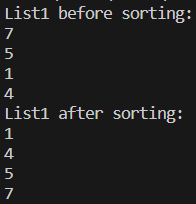
\includegraphics[width=0.25\textwidth]{Files/Billeder: Appendix/Insertion Sort Result.png}
    \end{center}
    \caption{The result for the insertion-sort code example}
    \label{figure:insetion_sort_result}
\end{figure}

\subsubsection{Code Example: Seconds Time-conversion} \label{acc_test_Seconds}

\subsubsection{Source Code in \lang:}
\begin{lstlisting}[language = scriptkid, firstnumber=1, label={list:acceptance_test_timeconversion_input}, caption=Acceptance test input of the timeconversion code example]
function mod(number a, number b) return number
{ 
    number remainder = a; 
    repeat while (remainder >= b) 
    { 
        remainder = remainder - b; 
    } 
    return remainder; 
} 
number seconds_in_minute = 60; 
number seconds_in_hour = seconds_in_minute * 60; 
number seconds_in_day = seconds_in_hour * 24; 
number seconds_in_week = seconds_in_day * 7; 
number input_seconds = call number input(); 
decimal weeks = input_seconds / seconds_in_week; 
input_seconds = call mod(input_seconds, seconds_in_week); 
decimal days = input_seconds / seconds_in_day; 
input_seconds = call mod(input_seconds, seconds_in_day); 
decimal hours = input_seconds / seconds_in_hour; 
input_seconds = call mod(input_seconds, seconds_in_hour); 
decimal minutes = input_seconds / seconds_in_minute; 
input_seconds = call mod(input_seconds, seconds_in_minute); 
call output("Number of weeks:"); 
call output(weeks); 
call output("Number of days:"); 
call output(days); 
call output("Number of hours:"); 
call output(hours);
call output("Number of minutes:"); 
call output(minutes); 
\end{lstlisting}

\subsubsection{Target Code in C:}
\begin{lstlisting}[language = c, firstnumber=106, label={list:acceptance_test_timeconversion_output}, caption=Acceptance test output of the timeconversion code example]
...
int mod(int a, int b) 
{ 
    int remainder = a; 
    while ((remainder >= b)) 
    { 
        remainder = (remainder - b); 
    } 
    return remainder; 
} 
void main() 
{ 
    int seconds_in_minute = 60; 
    int seconds_in_hour = (seconds_in_minute * 60); 
    int seconds_in_day = (seconds_in_hour * 24); 
    int seconds_in_week = (seconds_in_day * 7); 
    int input_seconds = *(int *)input("%d", sizeof(int)); 
    float weeks = (input_seconds / seconds_in_week); 
    input_seconds = mod(input_seconds, seconds_in_week); 
    float days = (input_seconds / seconds_in_day); 
    input_seconds = mod(input_seconds, seconds_in_day); 
    float hours = (input_seconds / seconds_in_hour); 
    input_seconds = mod(input_seconds, seconds_in_hour); 
    float minutes = (input_seconds / seconds_in_minute); 
    input_seconds = mod(input_seconds, seconds_in_minute); 
    printf("%s\n", "Number of weeks:"); 
    printf("%g\n", weeks); 
    printf("%s\n", "Number of days:"); 
    printf("%g\n", days); 
    printf("%s\n", "Number of hours:"); 
    printf("%g\n", hours); 
    printf("%s\n", "Number of minutes:"); 
    printf("%g\n", minutes); 
} 
\end{lstlisting}

\subsubsection{result:}

\begin{figure}[H] 
    \begin{center}
        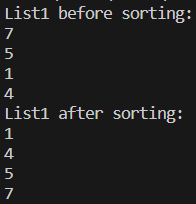
\includegraphics[width=0.25\textwidth]{Files/Billeder: Appendix/Insertion Sort Result.png}
    \end{center}
    \caption{The result for the time-conversion code example}
    \label{figure:timeconversion_result}
\end{figure}

\subsection{Code Example: GDB Calculator} \label{acc_test_Calcc}

\subsubsection{Source Code in \lang:}
\begin{lstlisting}[language = scriptkid, firstnumber=1, label={list:acceptance_test_GDB_input}, caption=Acceptance test input of the GDB calculator code example]
number divisor; 
number input_a; 
number input_b; 
number min; 
number max; 
number remainder; 
text tryAgain = "y"; 
function mod(number a, number b) return number 
{ 
    number remainder = a; 
    repeat while (remainder >= b) 
    { 
        remainder = remainder - b; 
    } 
    return remainder;   
} 
function GetMax() return number 
{ 
    if (input_a > input_b) 
    { 
        return input_a; 
    } 
    else 
    { 
        return input_b; 
    } 
    return -1; 
} 
function GetMin() return number 
{ 
    if (input_a < input_b) 
    { 
        return input_a; 
    } 
    else 
    { 
        return input_b; 
    } 
    return -1; 
} 
repeat while (tryAgain is "y") 
{ 
    comment: Asks for two positive integers as input and in the case of an error, ask the user again; 
    call output("Enter two positive integers:"); 
    boolean continue = false; 
    repeat while (continue is false) 
    { 
        input_a = call number input(); 
        input_b = call number input(); 
        if (input_a <= 0 or input_b <= 0) 
        { 
            call output("Please enter two positive integers:"); 
            continue = false; 
        } 
        else 
        { 
            continue = true; 
        } 
    } 
    max = call GetMax(); 
    min = call GetMin(); 
    continue = false; 
    number i = min; 
    repeat while(i > 0 and continue is false) 
    { 
        if (call mod(max, i) is 0 and call mod(min, i) is 0) 
        { 
            divisor = i; 
            continue = true; 
        } 
        i = i - 1; 
    } 
    call output("The biggest divisor is:"); 
    call output(divisor); 
    call output("Would you like to try again? (y/n)"); 
    tryAgain = call text input(); 
} 
\end{lstlisting}

\subsubsection{Target Code in C:}
\begin{lstlisting}[language = c, firstnumber=106, label={list:acceptance_test_timeconversion_output}, caption=Acceptance test output of the timeconversion code example]
...
int mod(int a, int b) 
{ 
    int remainder = a; 
    while((remainder >= b)) 
    { 
    remainder = (remainder - b); 
    } 
return remainder;
} 
int GetMax(int input_a, int input_b) 
{ 
    if((input_a > input_b)) 
    { 
        return input_a;
    } 
    else 
    { 
        return input_b;
    } 
    return -1;
} 
int GetMin(int input_a, int input_b) 
{ 
    if((input_a < input_b)) 
    { 
        return input_a;
    } 
    else 
    { 
        return input_b;
    } 
    return -1;
} 
void main(){ 
int divisor = 0; 
int input_a = 0; 
int input_b = 0; 
int min = 0; 
int max = 0; 
int remainder = 0; 
char * tryAgain = "y"; 
while(0 == strcmp(tryAgain, "y")) 
{ 
    printf("%s\n", "Enter two positive integers:"); 
    int continue_ = 0; 
    while((continue_ == 0)) 
    { 
    input_a = *(int *)input("%d", sizeof(int)); 
    input_b = *(int *)input("%d", sizeof(int)); 
        if(((input_a <= 0) || (input_b <= 0))) 
        { 
        printf("%s\n", "Please enter two positive integers:"); 
        continue_ = 0; 
        } 
        else 
        { 
        continue_ = 1; 
        } 
    } 
    max = GetMax(input_a, input_b); 
    min = GetMin(input_a, input_b); 
    continue_ = 0; 
    int i = min; 
    while(((i > 0) && (continue_ == 0))) 
    { 
    if(((mod(max, i) == 0) && (mod(min, i) == 0))) 
    { 
        divisor = i; 
        continue_ = 1; 
    } 
    i = (i - 1); 
    } 
    printf("%s\n", "The biggest divisor is:"); 
    printf("%d\n", divisor); 
    printf("%s\n", "Would you like to try again? (y/n)"); 
    tryAgain = (char *)input("%s", sizeof(char *));
    } 
} 
\end{lstlisting}

\subsubsection{result:}
\begin{figure}[H] 
    \begin{center}
        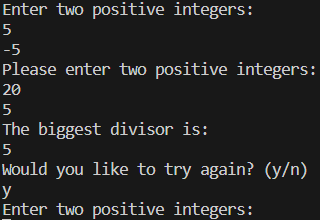
\includegraphics[width=0.40\textwidth]{Files/Billeder: Appendix/GDB Results.png}
    \end{center}
    \caption{The result for the GDB-calculator code example}
    \label{figure:repeatinput_result}
\end{figure}

\subsection{Code Example: test input \& repeat}

\subsubsection{Source Code in \lang:}
\begin{lstlisting}[language = scriptkid, firstnumber=1, label={list:acceptance_test_repeat_input_test}, caption=Acceptance test input of the repeat loops code example]
comment: Function to test repeat (x) times loop and input; 
function StartFunction() return nothing{
    text inputText; 
    boolean flag = true; 
    number repetitions; 
    repeat while(flag){ 
        call output(""); 
        call output("Write 'start' to start: "); 
        inputText = call text input(); 
        if(inputText is "start"){ 
            call output(""); 
            call output("Write amount of repetitions: "); 
            repetitions = call number input(); 
            repeat (repetitions) times{ 
                call output("This is a repeated message"); 
            }           
        } 
    } 
} 
call StartFunction(); 
\end{lstlisting}

\subsubsection{Target code in C:}
\begin{lstlisting}[language = C, firstnumber=106, label={list:acceptance_test_repeat_input_test_InC}, caption=Acceptance test input of the repeat loops code example output in C]
...
void StartFunction()
{
    char * inputText = "";
    int flag = 1;
    int repetitions = 0;
    while(flag){
        printf("%s\n", "");
        printf("%s\n", "Write 'start' to start: ");
        inputText = (char *)input("%s", sizeof(char *));
        if(0 == strcmp(inputText, "start")){
            printf("%s\n", "");
            printf("%s\n", "Write amount of repetitions: ");
            repetitions = *(int *)input("%d", sizeof(int));
            for (int number = 0; number < repetitions; number++){
               printf("%s\n", "This is a repeated message");
            }
        }
    }
}
void main(){
StartFunction();
}
\end{lstlisting}

\subsubsection{result:}
\begin{figure}[H] 
    \begin{center}
        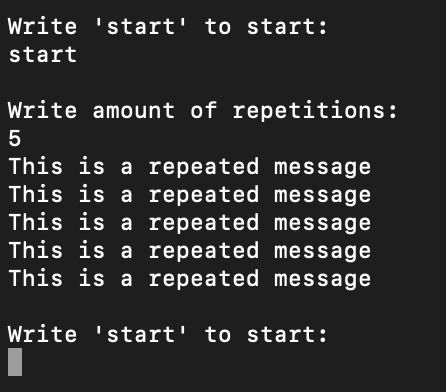
\includegraphics[width=0.40\textwidth]{Files/Billeder: Appendix/Repat And Input.png}
    \end{center}
    \caption{The result for the repeat-input code example}
    \label{figure:repeatinput_result}
\end{figure}




\subsection{Code Example: Triangle area calculate.}

\subsubsection{Source Code in \lang:}
\begin{lstlisting}[language = scriptkid, firstnumber=1, label={list:acceptance_test_triangle}, caption=Acceptance test calculating triangle code examples]
function triArea(number width, number height) return decimal
{ 
    return (width * height) / 2; 
} 
call output(call triArea(2,3)); 
call output(call triArea(7,4)); 
call output(call triArea(10,10)); 
call output(call triArea(3,3)); 
\end{lstlisting}



\subsubsection{Target code in C:}
\begin{lstlisting}[language = C, firstnumber=1, label={list:acceptance_test_triangle_output}, caption=Acceptance test triangle code examples in C]
float triArea(int width, int height)
{
    return ((width * height) / 2);
}
void main(){
printf("%g\n", triArea(2, 3));
printf("%g\n", triArea(7, 4));
printf("%g\n", triArea(10, 10));
printf("%g\n", triArea(3, 3));
}
\end{lstlisting}

\subsubsection{result:}
\begin{figure}[H] 
    \begin{center}
        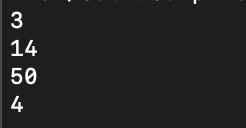
\includegraphics[width=0.40\textwidth]{Files/Billeder: Appendix/TriangleCalc.png}
    \end{center}
    \caption{The result for the calculate triangle area code example}
    \label{figure:triangleArea_result}
\end{figure}

\subsection{Mathematical Expressions} \label{test_MathExpr}

\subsubsection{Source Code in \lang:}
\begin{lstlisting}[language = scriptkid, firstnumber=1, label={list:acceptance_test_mathexpr}, caption=Acceptance test math expressions code examples]
number x = 14;
number y = 7;
number z = 10;

number A;
number B;
number C;
decimal D;
number E;

A = x + y;
B = x - y;
C = x * y;
D = x / y;
E = (x + y) * z;


call output(A);
call output(B);
call output(C);
call output(D);
call output(E);
\end{lstlisting}

\subsubsection{Target code in C:}
\begin{lstlisting}[language = C, firstnumber=1, label={list:acceptance_test_mathexpr_output}, caption=Acceptance test math expressions code examples in C]
void main(){
    int x = 14;
    int y = 7;
    int z = 10;
 
    int A = 0;
    int B = 0;
    int C = 0;
    float D = 0;
    int E = 0;
 
    A = (x + y);
    B = (x - y);
    C = (x * y);
    D = (x / y);
    E = ((x + y) * z);
 
    printf("%d\n", A);
    printf("%d\n", B);
    printf("%d\n", C);
    printf("%g\n", D);
    printf("%d\n", E);
}
\end{lstlisting}

\subsubsection{result:}
\begin{figure}[H] 
    \begin{center}
        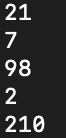
\includegraphics[width=0.10\textwidth]{Files/Billeder: Appendix/MathExpr.png}
    \end{center}
    \caption{The result for mathematical expressions code example}
    \label{figure:triangleArea_result}
\end{figure}

 number x = 5;
 text y = "this is a test"
 text z = 5;

 \subsection{Missing ";" error message} \label{test_MissingSemi}

\subsubsection{Source Code in \lang:}
\begin{lstlisting}[language = scriptkid, firstnumber=1, label={list:acceptance_test_missingsemi}, caption=Acceptance test missing ";" code examples]
 number x = 5;
 text y = "this is a test"
 text z = 5;
\end{lstlisting}

\subsubsection{result:}
\begin{figure}[H] 
    \begin{center}
        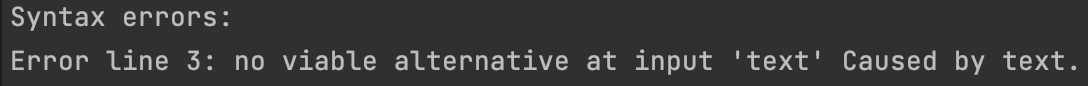
\includegraphics[width=1\textwidth]{Files/Billeder: Appendix/errormsg1.png}
    \end{center}
    \caption{The result for missing semi colon code example}
    \label{figure:errorMsg1_result}
\end{figure}


 \subsection{Wrong type error message} \label{test_TypeErr}
\subsubsection{Source Code in \lang:}
\begin{lstlisting}[language = scriptkid, firstnumber=1, label={list:acceptance_test_wrongtype}, caption=Acceptance wrong type code examples]
text y = "a";
text z = 5;
 \end{lstlisting}

 \subsubsection{result:}
\begin{figure}[H] 
    \begin{center}
        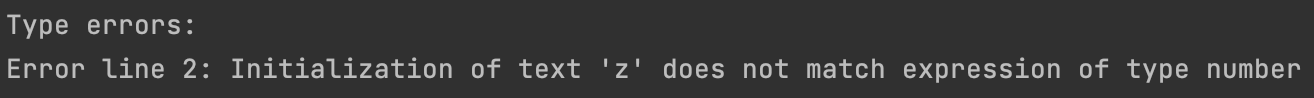
\includegraphics[width=1\textwidth]{Files/Billeder: Appendix/errormsg2.png}
    \end{center}
    \caption{The result for wrong type code example}
    \label{figure:errorMsg2_result}
\end{figure}


\subsection{String Concatenation} \label{test_stringconc}

\subsubsection{Source Code in \lang:}
\begin{lstlisting}[language = scriptkid, firstnumber=1, label={list:acceptance_test_stringconc}, caption=Acceptance test string conc code examples]
text hej = "gem" + "fem";

call output(hej);
\end{lstlisting}

\subsubsection{Target code in C:}
\begin{lstlisting}[language = C, firstnumber=1, label={list:acceptance_test_stringconc_output}, caption=Acceptance test string conc code examples in C]
char* concat(const char *str1, const char *str2) 
{
     size_t len1 = strlen(str1);
     size_t len2 = strlen(str2);
     char *result = malloc(strlen(str1) + strlen(str2) + 1);
     strcpy(result, str1);
     strcat(result, str2);
     return result;
}

void main()
{
    char * hej = concat("gem", "fem");
    printf("%s\n", hej);
}

\end{lstlisting}

 \subsubsection{result:}
\begin{figure}[H] 
    \begin{center}
        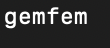
\includegraphics[width=0.2\textwidth]{Files/Billeder: Appendix/stringconc.png}
    \end{center}
    \caption{The result for string concatenation code example}
    \label{figure:stringconc_result}
\end{figure}


\subsection{Zero Division}

\subsubsection{Source Code in \lang:}
\begin{lstlisting}[language = scriptkid, firstnumber=1, label={list:acceptance_test_zerodiv}, caption=Acceptance test division by zero code examples]
number x = 5;
number y = 0;
decimal a;
decimal b;

a = x / y;
b = y / x ;


call output(a);
call output(b);
\end{lstlisting}

\subsubsection{Target code in C:}
\begin{lstlisting}[language = C, firstnumber=1, label={list:acceptance_test_zerodiv_output}, caption=Acceptance test division by zero code examples in C]
void main()
{
    int x = 5;
    int y = 0;
    float A = 0;
    float B = 0;
    
    A = (divide(x, y));
    B = (divide(y, x));
    
    printf("%g\n", A);
    printf("%g\n", B);
}
\end{lstlisting}


 \subsubsection{result:}
\begin{figure}[H] 
    \begin{center}
        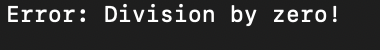
\includegraphics[width=0.4\textwidth]{Files/Billeder: Appendix/ZeroDiv.png}
    \end{center}
    \caption{The result for division by zero code example}
    \label{figure:zerodiv_result}
\end{figure}

\subsection{Symbol Table scope-fix}
\label{Appendix:ScopeFix}

\subsubsection{AddIdToFunctionBlock:}
\begin{lstlisting}[language = csharp, firstnumber=232, label={list:symbolTable_AddIdToFunction}, caption=AddIdToFunctionBlock - 134-169 - CobraCompiler/SymbolTable.cs]
public void AddIDToFunctionBlock(Symbol symbol, BlockNode blockNode)
{
    //Only add the ID if the ID is contained in a functionBlock
    //and has not already been declared within this functionBlock

    FunctionBlockNode? fBlockNode = null;

    var scope = _scopes[blockNode];

    while (scope != null)
    {
        //Has functionBlock:
        if (scope.Block is FunctionBlockNode)
        {
            fBlockNode = scope.Block as FunctionBlockNode;
        }

        //If the name is declared within the current scope, we don't add it
        if (scope.Symbols.ContainsKey(symbol.Name))
            break;

        //If has functionBlock and has not been declared yet in any scopes,
        //The ID must've been an identifier from outside the function
        if (fBlockNode != null)
        {

            if (!fBlockNode.UsedVariables.Keys.Contains(symbol.Name))
                fBlockNode.UsedVariables.Add(symbol.Name, symbol.Type);

            //Exit because we've now met a functionBlockNode
            break;
        }

        scope = scope.Parent;
    }
}
\end{lstlisting}

\subsubsection{Visit Declaration-Node:}
\begin{lstlisting}[language = csharp, firstnumber=232, label={list:symbolTable_DeclarationNode}, caption=Visit Declaration-Node - 232-250 - CobraCompiler/SymbolTable.cs]
public override ASTNode? Visit(DeclarationNode node)
{
    if (_reservedKeywords.Contains(node.Identifier.Name))
        node.Identifier.Name = $"{node.Identifier.Name}_";

    var sym = Lookup(node.Identifier.Name, _currentBlock);

    string underscores = "";
    while (sym != null)
    {
        underscores += "_";
        sym = Lookup($"{node.Identifier.Name}{underscores}", _currentBlock);
    }

    node.Identifier.Name += underscores;
    Insert(node.Identifier.Name, node.Identifier.TypeNode.Type, node);
    Visit(node.Expression);
    return null;
}
\end{lstlisting}

\subsubsection{Visit Identifier-Node:}
\begin{lstlisting}[language = csharp, firstnumber=767, label={list:symbolTable_IdentifierNode}, caption=Visit Identifier-Node - 767-792 - CobraCompiler/SymbolTable.cs]
public void Visit(IdentifierNode node)
{
    if (_reservedKeywords.Contains(node.Name))
        node.Name = $"{node.Name}_";

    var prevSym = Lookup(node.Name, _currentBlock);
    var currSym = Lookup($"{node.Name}_", _currentBlock);

    string underscores = "_";
    while (currSym != null)
    {
        prevSym = currSym;
        currSym = Lookup($"{node.Name}{underscores}", _currentBlock);
        underscores += "_";
    }

    node.Name = prevSym.Name;

    if (prevSym != null)
        AddIDToFunctionBlock(prevSym, _currentBlock);

    if (prevSym == null)
    {
        SymbolError(node, $"{node.Name} is not found. Declare your variable before use.");
    }
}
\end{lstlisting}